%%%%%%%%%%%%%%%%%%%%%%%%%%%%%%%%%%%%%%%%%
% Beamer Presentation
% LaTeX Template
% Version 1.0 (10/11/12)
%
% This template has been downloaded from:
% http://www.LaTeXTemplates.com
%
% License:
% CC BY-NC-SA 3.0 (http://creativecommons.org/licenses/by-nc-sa/3.0/)
%
%%%%%%%%%%%%%%%%%%%%%%%%%%%%%%%%%%%%%%%%%

%----------------------------------------------------------------------------------------
%	PACKAGES AND THEMES
%----------------------------------------------------------------------------------------

\documentclass[9pt]{beamer}

\mode<presentation> {

% The Beamer class comes with a number of default slide themes
% which change the colors and layouts of slides. Below this is a list
% of all the themes, uncomment each in turn to see what they look like.

%\usetheme{default}
%\usetheme{AnnArbor}
%\usetheme{Antibes}
%\usetheme{Bergen}
%\usetheme{Berkeley}
%\usetheme{Berlin}
%\usetheme{Boadilla}
%\usetheme{CambridgeUS}
%\usetheme{Copenhagen}
%\usetheme{Darmstadt}
%\usetheme{Dresden}
%\usetheme{Frankfurt}
%\usetheme{Goettingen}
%\usetheme{Hannover}
%\usetheme{Ilmenau}
%\usetheme{JuanLesPins}
%\usetheme{Luebeck}
\usetheme{Madrid}
\usepackage{caption}
\usepackage{subcaption}
\usepackage{epigraph}
%\usetheme{Malmoe}
%\usetheme{Marburg}
%\usetheme{Montpellier}
%\usetheme{PaloAlto}
%\usetheme{Pittsburgh}
%\usetheme{Rochester}
%\usetheme{Singapore}
%\usetheme{Szeged}
%\usetheme{Warsaw}

% As well as themes, the Beamer class has a number of color themes
% for any slide theme. Uncomment each of these in turn to see how it
% changes the colors of your current slide theme.

%\usecolortheme{albatross}
%\usecolortheme{beaver}
%\usecolortheme{beetle}
%\usecolortheme{crane}
%\usecolortheme{dolphin}
%\usecolortheme{dove}
%\usecolortheme{fly}
%\usecolortheme{lily}
%\usecolortheme{orchid}
%\usecolortheme{rose}
%\usecolortheme{seagull}
%\usecolortheme{seahorse}
%\usecolortheme{whale}
%\usecolortheme{wolverine}
\usecolortheme{rose}

%\setbeamertemplate{footline} % To remove the footer line in all slides uncomment this line
%\setbeamertemplate{footline}[page number] % To replace the footer line in all slides with a simple slide count uncomment this line

%\setbeamertemplate{navigation symbols}{} % To remove the navigation symbols from the bottom of all slides uncomment this line
}

\usepackage{graphicx} % Allows including images
\usepackage{booktabs} % Allows the use of \toprule, \midrule and \bottomrule in tables
\usepackage{hyperref}
\usepackage{scalerel,stackengine}
\usepackage[ruled,vlined]{algorithm2e}
\usepackage{algorithm,algpseudocode}
\usepackage{caption}
\usepackage{subcaption}
% \usepackage{algorithm}
\usepackage{algorithmic}
\stackMath
\newcommand\reallywidehat[1]{%
\savestack{\tmpbox}{\stretchto{%
  \scaleto{%
    \scalerel*[\widthof{\ensuremath{#1}}]{\kern-.6pt\bigwedge\kern-.6pt}%
    {\rule[-\textheight/2]{1ex}{\textheight}}%WIDTH-LIMITED BIG WEDGE
  }{\textheight}% 
}{0.5ex}}
\stackon[1pt]{#1}{\tmpbox}%
}
\parskip 1ex
%----------------------------------------------------------------------------------------
%	TITLE PAGE
%----------------------------------------------------------------------------------------

\title[CS769 Optimization in ML]{Learning Heuristics to solve Travelling Salesmen problem} % The short title appears at the bottom of every slide, the full title is only on the title page

\author{Tejas Pagare, Kaustubh Ponkshe} % Your name
\institute[IIT Bombay] % Your institution as it will appear on the bottom of every slide, may be shorthand to save space
{ CS769 Paper Presentation\\
% \medskip
%  \textit{\href{mailto:tejaspagare2002@gmail.com}{tejaspagare2002@gmail.com} } \\%\textit{School of Management} \\ % Your institution for the title page
\medskip
%\textit{bofu20131@163.com} % Your email address
% {Prof. Vivek Borkar}\\

{Electrical Engineering Department}\\
{Indian Institute of Technology Bombay}\\
\vspace{10pt}\\

}
\date{\today} % Date, can be changed to a custom date

\begin{document}

\begin{frame}
\titlepage % Print the title page as the first slide
\end{frame}

\begin{frame}
\frametitle{Outline} % Table of contents slide, comment this block out to remove it
\tableofcontents % Throughout your presentation, if you choose to use \section{} and \subsection{} commands, these will automatically be printed on this slide as an overview of your presentation
\end{frame}

%----------------------------------------------------------------------------------------
%	PRESENTATION SLIDES
%----------------------------------------------------------------------------------------

%------------------------------------------------
% \section{Average Reward Formulation} % Sections can be created in order to organize your presentation into discrete blocks, all sections and subsections are automatically printed in the table of contents as an overview of the talk
%------------------------------------------------

\section{Introduction}

\section{Travelling Salesman Problem}

\section{Heuristic Methods}

\section{Learning Based Methods}
\section{Experimental Results}
\section{Future Direction}
\begin{frame}{Combinatorial Optimization}
\vspace{-40pt}
% Lot of prior algorithms were Heuristic based.
% \bigskip\\
% Can we learn such heuristic algorithms?\\ 
% \begin{center}
%     Yes, using Machine Learning!
% \end{center}
\begin{itemize}
\item Combinatorial optimization is an optimization
problem wit discrete objects and the objective of the algorithm is to minimize or maximize a cost function.\\
\vspace{20}
\item The problem is to find an optimal solution from a feasible set of discrete finite solutions. \\
\vspace{20}
\item Some examples of
combinatorial optimization include Travelling salesman-problem, minimum graph cut, set cover problem, etc
\end{itemize}
\end{frame}

% We need to represent the graph nodes using features and learning a Machine Learning algorithm on the features.
% \\
% \bigskip\\
\begin{frame}{Applications}

\centering
    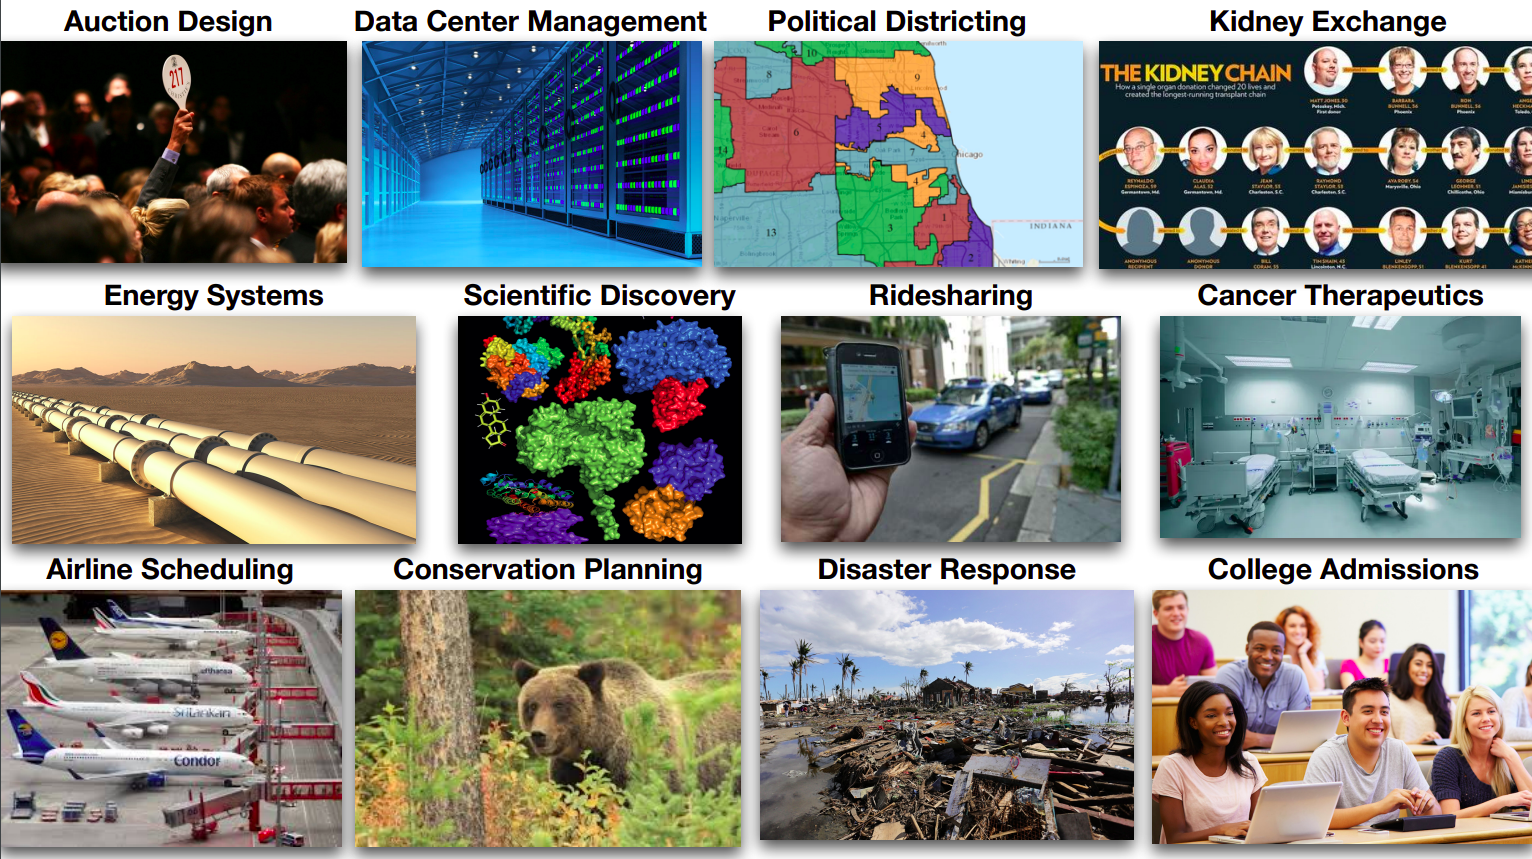
\includegraphics[width=0.8\textwidth]{images/Applications.png}
\end{frame}


\begin{frame}{Travelling Salesman Problem}
% \vspace{-40pt}
\begin{definition}[Travelling Salesman Problem]

\emph{"Given a set of points in 2-dimensional space, find a tour
of minimum total weight, where the corresponding graph G has the points as nodes and is fully
connected with edge weights corresponding to distances between points; a tour is a cycle that visits each node of the graph exactly once"}

\end{definition}
Consider a graph $G= (V,E) $ where $V = (v_1, v_2, ...v_n)$ is a set of n vertices and there is a cost function $c_{ij}$ associated with each edge $e_{ij} \in E$. Now consider variables $x_{ij}$ such that .
$$ 
x_{ij} =
\begin{cases}
    1 \text{  if there is a path from i to j}\\    
 0  \text{  otheriwse}
\end{cases} $$
Then our optimization problem can be given as 
$$ \text{min } \sum_{i=1}^n  \sum_{i \neq j,j=1}^n x_{ij}c_{ij}$$
with the constraint that 
$$  \sum_{i=1,i \neq j}^n x_{ij}=1, \text{ for every $j$ and }  \sum_{i \neq j,j=1}^n x_{ij}=1  \text{ for every $i$} $$
\end{frame}
\begin{frame}{Greedy Methods}
% \vspace{-40pt}
Greedy algorithms are a class of algorithms which look for best in the short run, whether or not it is best in the long run.Greedy algorithms optimize locally, but not necessarily globally.
\begin{definition}[Nearest Neighbour Algorithm]

\emph{"The Nearest-Neighbor Algorithm begins at any vertex and follows the
edge of least weight from that vertex. At every subsequent vertex, it
follows the edge of least weight that leads to a city not yet visited, until
it returns to the starting point."}

\end{definition}

\end{frame}
\begin{frame}{Heursitic Based Methods}
% \vspace{-40pt}
A heuristic function, also simply called a heuristic, is a function that ranks alternatives in search algorithms at each branching step based on available information to decide which branch to follow.
\begin{algorithm}[H]

\SetAlgoLined
\textbf{Select} $v_1\in V,\text{Intitialize subgraph}\ S= \phi$\\
\text{Find vertex} $v_j = \text{argmin}_j c_{1j}$ \\
$S= {v_1,v_j,v_1}$\\
\For{t=1 to n-2}{
  Find vertex $v_k = \text{argmin}_{v_i \in S} c_{ik}$\\
  \text{Find arc} (i,j) = \text{argmin}_{v_i \in S} c_{ik} + c_{jk}- c_{ij}\\
  \text{Update}  S= {v_1,v_{k1},....,v_j,v_k,v_i...}

 }
 \EndFor
 \caption{Nearest Insertion Algorithm}

\end{algorithm}
Farthest Insertion Algorithm inserts farthest points
\end{frame}
\begin{frame}{Average and Worst case results}
\begin{itemize}
    \item \textbf{Nearest Neighbour:} Average length = 1.26*length of optimal tour, no worst case bound
    \vspace{20pt}
    \item \textbf{Nearest Insertion:} worst case length = 2*length of optimal tour, $O(n^2)$ complexity
    \vspace{20pt}
    \item \textbf{Farthest Insertion:} worst case length = 2*log(n)*length of optimal tour, $O(n^2)$ complexity
\end{itemize}
\end{frame}
\begin{frame}{Experimental Results}
\vspace{-60pt}
\begin{center}
\begin{tabular}{|c|c|c|c|}
\hline
    Nodes & Nearest Neighbour &  Nearest Insertion & Farthest Insertion\\\hline
    20 & 5.106 & 5.248 & 5.246\\\hline
    50 & 7.293  & 7.378 & 8.076\\\hline
\end{tabular}
\end{center}

\end{frame}
\begin{frame}{Learning Based Methods}
\vspace{-40pt}
Lot of prior algorithms were Heuristic based.
\bigskip\\
Can we learn such heuristic algorithms?\\ 
\begin{center}
    Yes, using Machine Learning!
\end{center}

% We need to represent the graph nodes using features and learning a Machine Learning algorithm on the features.
% \\
% \bigskip\\
Problem Statement:
\begin{center}
    Given a graph optimization problem $G$
and a distribution $D$ of problem instances,
can we learn better greedy heuristics that
generalize to unseen instances from $D$?
\end{center}

\end{frame}
\begin{frame}{Reinforcement Learning}
\begin{tabular}{cc}
     Greedy Algorithm & Reinforcement Learning  \\
     \textcolor{blue}{Partial solution}&State\\
     \textcolor{green}{Scoring function}&Q-function\\
Select \textcolor{red}{best node} &Greedy Policy
\end{tabular}
\bigskip\\
Algorithm:\\
Repeat until all edges are covered:
\begin{enumerate}
    \item Compute node \textcolor{green}{scores}
\item Select \textcolor{red}{best node} w.r.t. \textcolor{green}{score}
\item Add \textcolor{red}{best node} to \textcolor{blue}{partial solution}.
\end{enumerate}
\end{frame}

\begin{frame}{Markov Decision Process}
% \vspace{-40pt}
\begin{definition}[Markov Decision Process]
A MDP consists of 
\begin{itemize}
    \item A set of states $\mathcal{S}$, set of actions $\mathcal{A}$ for moving from a state to another. $\mathcal{S}$ and $\mathcal{A}$ can be both finite or infinite.
    \item Transition Probabilities $P$: probability distribution over next states given the current state and current action where $P_{ij}(a) = \text{Pr}\{X_{n+1}=j|X_{n}=i,U_n=a\}$.
    \item A reward function: $\mathcal{R}: \mathcal{S}\times\mathcal{A}\rightarrow\mathbb{R}$, where $\mathcal{R}_s^a$ or $r(s,a)$ is the expected reward of taking action $a$ in state $s$.
\end{itemize} 
Therefore a MDP is simply given as a pair $(\mathcal{S},\mathcal{A},P,\mathcal{R})$.\\
\end{definition}
\end{frame}

\begin{frame}{Reinforcement Learning (contd.)}
\begin{figure}[H]
    \centering
    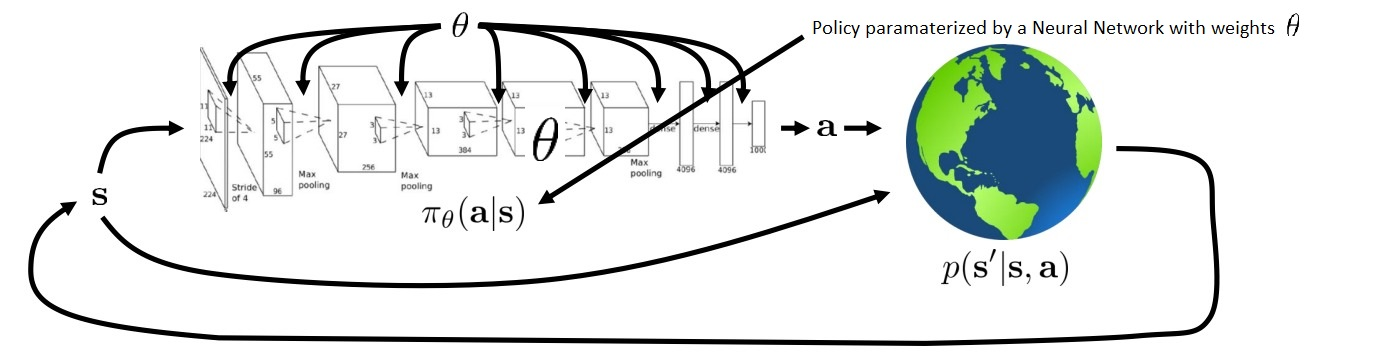
\includegraphics[width=10cm]{images/rl.jpeg}
    \caption{Environment-Agent Interaction}
    \label{fig:my_label}
\end{figure}
We usually consider learning in a Markov Decision Process $(\mathcal{S},\mathcal{A},P,\mathcal{R})$ where the aim is to find
\[\theta^\star = \underset{\theta}{\text{argmax}}\mathbb{E}_{\tau\sim p_\theta(\tau)}\Big[\sum_t r(s_t,a_t)\Big]\]
where 
\[p_\theta(s_1,a_t,\ldots,s_T,a_T)=p(s_1)\prod_{t=1}^T\pi_\theta(a_t|s_t)p(s_{t+1}|s_t,a_t)\]
\end{frame}


\begin{frame}{REINFORCE Algorithm}
\begin{theorem}[Policy Gradient Theorem]
\begin{equation}
\label{eq:pg}
    \nabla J(\theta) \propto \sum_s \mu(s) \sum_a\Big(Q_\pi(s,a)-b(s)\Big)\nabla \pi_\theta(a|s)
\end{equation}
where $J(\theta)=\mathbb{E}_{\tau\sim p_\theta(\tau)}\Big[\sum_t r(s_t,a_t)\Big]$ and \[Q_\pi(s,a)=\mathbb{E}_\pi[G_t|S_t=s,A_t=a]=\mathbb{E}_\pi\Big[\sum_{k=0}^\infty\gamma^k R_{t+k+1}|S_t=s,A_t=a\Big]\]
is the Q-value function for policy $\pi$ and $\mu(s)$ is a state distribution satisfying $\mu(s)\geq0\ \forall\ s$ and $\sum_s\mu(s)=1$.
\end{theorem}
The policy-gradient methods seek to maximize $J$ as follows:
\[\theta_{t+1}=\theta_t+\alpha\reallywidehat{\nabla J(\theta_t)}\]
where $\reallywidehat{\nabla J(\theta_t)}$ is the stochastic estimate of the actual gradient of $J$ w.r.t  $\theta$.
    
\end{frame}

\begin{frame}{REINFORCE Algorithm (contd.)}
\begin{algorithm}[H]
\SetAlgoLined
\caption{REINFORCE with Baseline (episodic), for estimating $\pi_\theta\approx\pi_*$}
\textbf{Input}: a differentiable policy parameterization $\pi_\theta(a|s)$, a differentiable state-value function parameterization $\hat{V}(s,w)$\\
Algorithm parameters: step sizes $\alpha_1 > 0, \alpha_2 > 0$\\
Initialize policy parameter $\theta\in\mathbb{R}^{d'}$ and state-value parameters $w\in\mathbb{R}^d$\\
\For{\text{each episode}}{
Generate an episode $S_0, A_0, R_1,\ldots,S_{T-1},A_{T-1},R_T,$ following $\pi_\theta(\cdot|\cdot)$\\
\For{\text{step} t=0,1,\ldots,T-1}{
$G\gets \sum_{k=t+1}^T\gamma^{k-t-1}R_k$\\
$\delta\gets G-\hat{V}(s,w)$\\
$w\gets w+\alpha_1\delta\nabla\hat{V}(S_t,w)$\\
$\theta\gets\theta+\alpha_2\gamma^t\delta\nabla\text{ln}\pi_\theta(A_t|S_t)$
}}
\end{algorithm}
\end{frame}

\begin{frame}{Attention, Learn to Solve Routing Problems!}
Consider for the n-node graph problem instance $s$, the solution tour $\pi = (\pi_1,\ldots,\pi_n)$ as the permutation of nodes, $\pi_t\in\{1,\ldots,n\}$. The aim is to find a stochastic policy factorized using $p_\theta(\pi|s)=\prod_{t=1}^n p_\theta(\pi_t|s,\pi_{1:t-1})$.
\bigskip\\
Here, we consider the an encoder-decoder architecture similar to Transformer (Vaswani et al., 2017).
\begin{figure}[H]
    \centering
    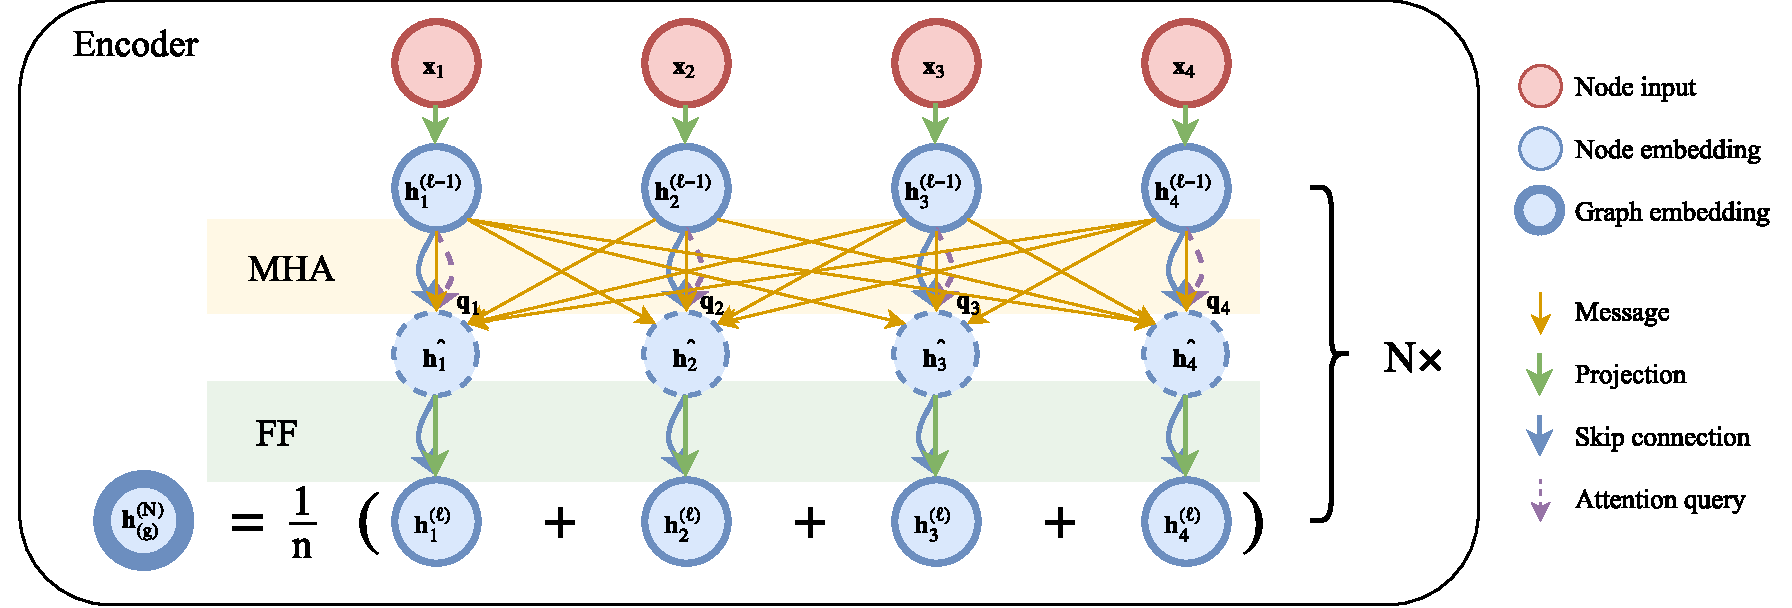
\includegraphics[width=8cm]{images/Encoder.pdf}
    \caption{Attention based encoder}
    \label{fig:my_label}
\end{figure}
$x_i$: $d_x$ dimensional input feature for node $i$\\
$h_i^{(0)}:$ learned $d_h$ dimensional node embedding\\
Output: node embedding for each node $i$, $h_i^{(N)}$ and graph embedding $\bar h ^{(N)}=\dfrac{1}{n}\sum_{i=1}^n h_i^{(N)}$
\end{frame}

\begin{frame}{Attention Based Algorithm (contd.)}
\begin{figure}[H]
    \centering
    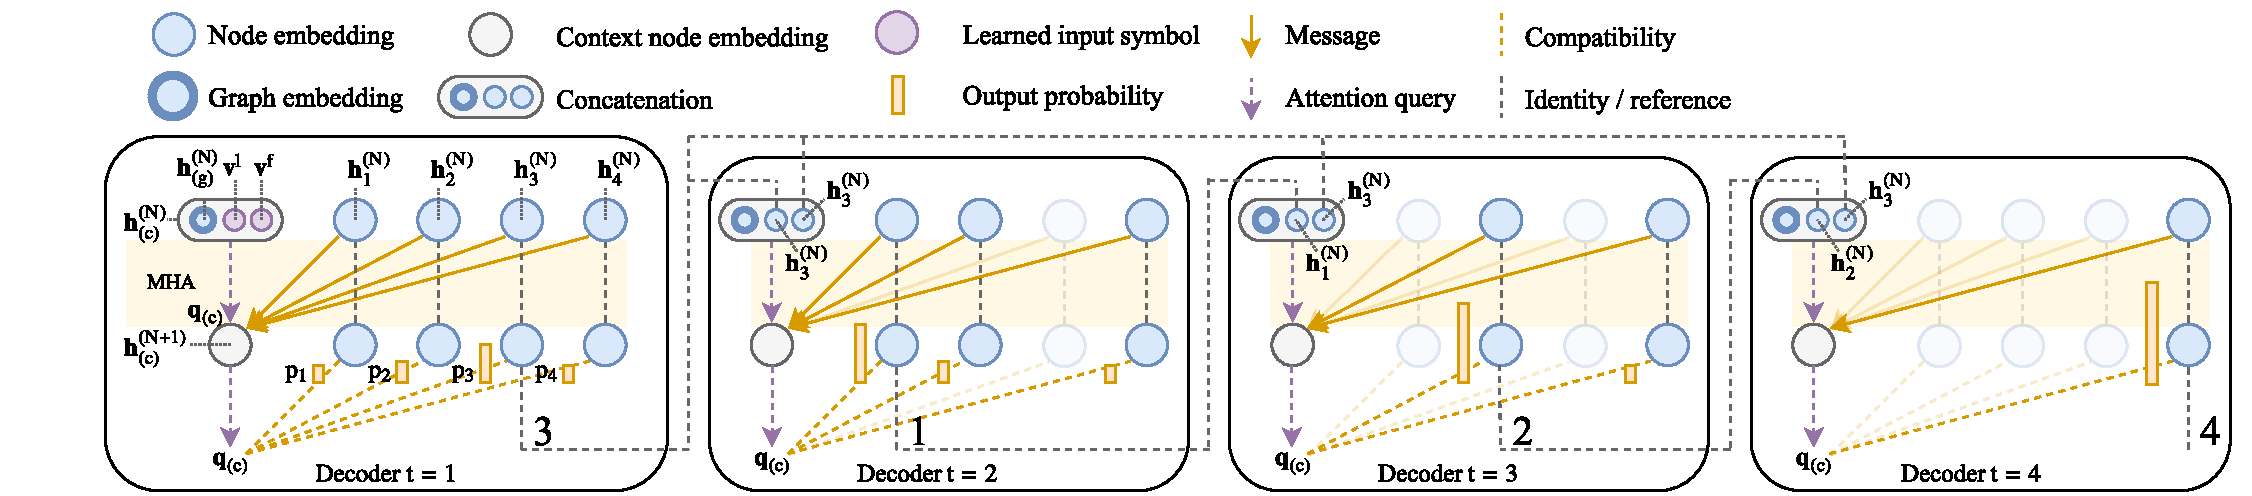
\includegraphics[width=10cm]{images/Decoder.pdf}
    \caption{Decoder with output tour as (3,1,2,4)}
    \label{fig:my_label}
\end{figure}    
Context Encoding:
\begin{equation*}
	
\begin{tabular}{cc}
     \mathbf{h}_{(c)}^{(N)} = \begin{cases}
		\left[\bar{\mathbf{h}}^{(N)} , \mathbf{h}^{(N)}_{\pi_{t-1}} , \mathbf{h}^{(N)}_{\pi_1}\right] & t > 1 \\
        \left[\bar{\mathbf{h}}^{(N)}, \mathbf{v}^\text{l}, \mathbf{v}^\text{f}\right] & t = 1
\end{cases} & 	\mathbf{q}_{(c)} = W^Q \mathbf{h}_{(c)},  \mathbf{k}_i = W^K \mathbf{h}_i,  \mathbf{v}_i = W^V \mathbf{h}_i \\
u_{(c)j} = \begin{cases}
		C \cdot \tanh \left(\frac{\mathbf{q}_{(c)}^T \mathbf{k}_j}{\sqrt{d_{\text{k}}}}\right) & \text{if } j \neq \pi_{t'} \quad \forall t' < t \\
        -\infty & \text{otherwise}
    \end{cases} &p_i = p_{\bm{\theta}}(\pi_t = i|s, \bm{\pi}_{1:t-1}) = \frac{e^{u_{(c)i}}}{\sum_{j}{e^{u_{(c)j}}}}
\end{tabular}
\end{equation*}
where $u_{(c)j}$ are called compatibilities.
\end{frame}

\begin{frame}{Using REINFORCE}
From the probability distribution $p_\theta(\pi|s)$ obtained from the decoder for the problem instance $s$, we sample a policy $\pi$ (permutation of nodes) to computed the loss defined as\\
\[\mathcal{L}(\theta|s)=\mathbb{E}_{p_\theta(\pi|s)}[L(\pi)]\]
For REINFORCE we have the gradient of the loss as
\[\nabla\mathcal{L}(\theta|s)=\mathbb{E}_{p_\theta(\pi|s)}[(L(\pi)-b(s))\nabla \text{log}p_\theta(\pi|s)]\]

A good baseline $b(s)$ reduces the gradient variance!\\
We use 2 baselines for the experimentation:
\begin{enumerate}
    \item greedy rollout baseline: defined as the cost of a solution of a deterministic greedy rollout policy by the best model so far
    \item critic: a function $\hat{V}{s,w}$ of state $s$, parameterized by $w$, which is learned using gradient ascent iteration similar to original REINFORCE iteration
\end{enumerate}
\end{frame}
\begin{frame}{More on Baseline}
    During the model training, the baseline is frozen for fixed number of steps every epoch.
    
    \bigskip\\
    
    The parameters associated with baseline policy $\bm{\theta}^{\text{BL}}$ is changed to policy parameters $\theta$ at the end of every epoch if current training policy is better compared to the baseline policy according to a paired t-test. 
\end{frame}
\begin{frame}{Overall Algorithm}
\begin{algorithm}[H]
\SetAlgoLined
  \caption{REINFORCE with Rollout Baseline} \label{alg:reinforce_rollout}
  \textbf{Input:}number of epochs $E$, steps per epoch $T$, batch size $B$, significance $\alpha$\\
    Init $\bm{\theta},\ \bm{\theta}^{\text{BL}} \gets \bm{\theta}$\\
      \For{$\text{epoch} = 1, \ldots, E$}{
        \For{$\text{step} = 1, \ldots, T$}{
        	 $s_i \gets \text{RandomInstance()} \enspace \forall i \in \{1, \ldots, B\}$\\
             $\bm{\pi}_i \gets \text{SampleRollout}(s_i, p_{\bm{\theta}}) \enspace \forall i \in \{1, \ldots, B\}$\\ $\bm{\pi}_i^{\text{BL}} \gets \text{GreedyRollout}(s_i, p_{\bm{\theta}^{\text{BL}}}) \enspace \forall i \in \{1, \ldots, B\}$\\ $\nabla\mathcal{L} \gets \sum_{i=1}^{B} \left(L(\bm{\pi}_i) - L(\bm{\pi}_i^{\text{BL}})\right) \nabla_{\bm{\theta}} \log p_{\bm{\theta}}(\bm{\pi}_i)$\\
             $\bm{\theta} \gets \text{Adam}(\bm{\theta}, \nabla\mathcal{L})$}

      \If{$\text{OneSidedPairedTTest}(p_{\bm{\theta}}, p_{\bm{\theta}^{\text{BL}}}) < \alpha$}{
		 $\bm{\theta}^{\text{BL}} \gets \bm{\theta}$}}
\end{algorithm}   
\end{frame}



\begin{frame}{Experimental Results}
\begin{figure}[H]
\captionsetup[subfigure]{justification=centering}
     \centering
    \begin{subfigure}{0.48\linewidth}
         \centering
         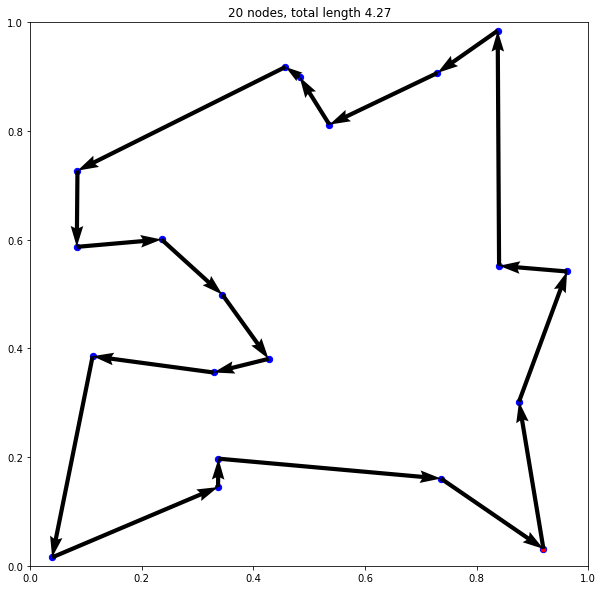
\includegraphics[width=0.9\linewidth]{images/learned_20.png}
         \caption{20 Nodes}
        \label{fig:bandit}
     \end{subfigure}
      \begin{subfigure}{0.48\linewidth}
         \centering
         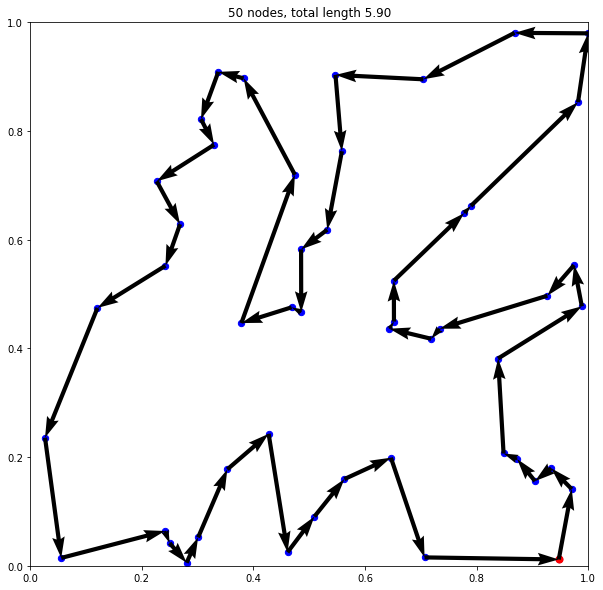
\includegraphics[width=0.9\linewidth]{images/learned_50.png}
         \caption{50 Nodes}
        %  \label{fig:nonideal}
     \end{subfigure}
     \caption{Solving Traveling Salesman Problem}
\end{figure}    
\end{frame}

\begin{frame}{Experimental Results (contd.)}

\end{frame}

\begin{frame}{Experimental Results (contd.)}
\begin{figure}[H]
    \centering
    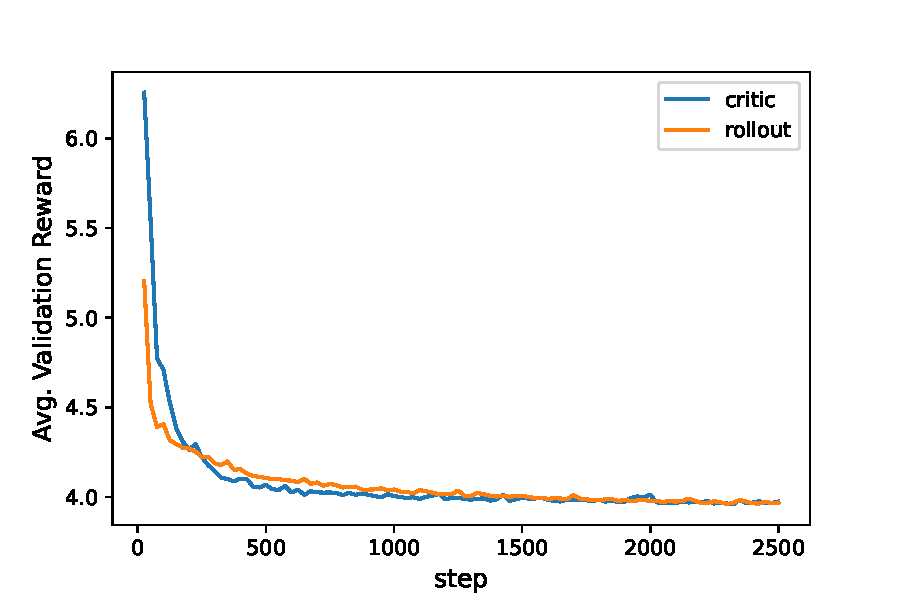
\includegraphics[width=5cm]{images/rollout-critic.pdf}
    \caption{Different baseline: greedy rollout and critic}
    \label{fig:my_label}
\end{figure}
\vspace{-20pt}
\begin{figure}[H]
\captionsetup[subfigure]{justification=centering}
     \centering
    \begin{subfigure}{0.48\linewidth}
         \centering
         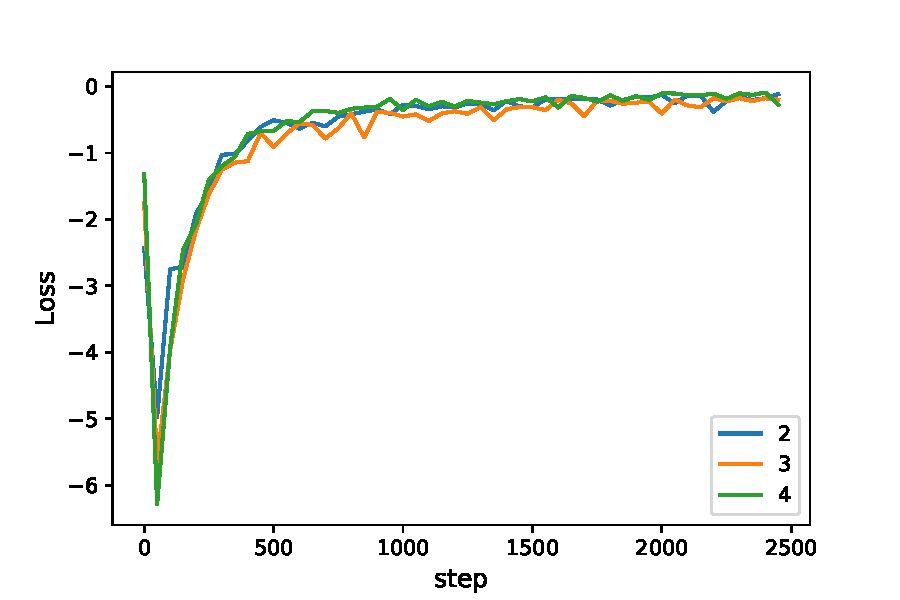
\includegraphics[width=0.9\linewidth]{images/layerloss.pdf}
         \caption{Learning Loss}
        \label{fig:bandit}
     \end{subfigure}
      \begin{subfigure}{0.48\linewidth}
         \centering
         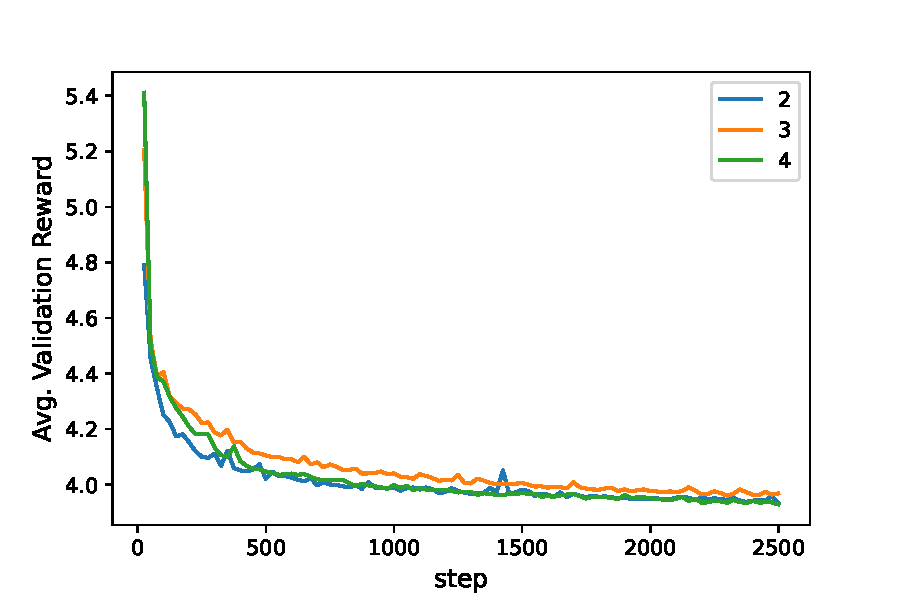
\includegraphics[width=0.9\linewidth]{images/layerreward.pdf}
         \caption{Average Reward}
        %  \label{fig:nonideal}
     \end{subfigure}
     \caption{Different Encoder Layers}
\end{figure}


\end{frame}






\begin{frame}

\Huge{\centerline{The End}}
\end{frame}


\end{document} 